\subsection{Parallel BO}
%----------------------------------------------------------------------
%----------------------------------------------------------------------
\begin{frame}[c]{Parallel BO}

\begin{itemize}
    \item Can we determine which $\conf$ to evaluate next, while other points are being evaluated? \pause
    \item \emph{Idea}: Utilize tractable properties of GP to get Monte Carlo estimates of acquisition function under different results from pending function evaluations. \pause
    \item Consider the case where $N$ evaluations have completed, with data $\left \{\bonextsample, \bonextobs \right \}^{N}_{\bocount = 1}$ and $J$ evaluations are pending $\left \{\conf_{j} \right \}^{J}_{j = 1}$: \pause
    \begin{equation*}
        \begin{aligned}
            \hat{\acq} ( \conf; \left \{ \bonextsample, \bonextobs \right \}, \left \{ \conf_j \right \} ) =  \pause
            \int_{\mathbb{R}^J}  \pause \acq ( \conf; \left \{ \bonextsample, \bonextobs \right \}, \left \{ \conf_j, \boobs_j \right \} ) \\  \pause
            p(\left \{ \boobs_j \right \}^{J}_{j = 1}  \rvert \left \{ \conf_j \right \}^{J}_{j = 1}, \left \{ \bonextsample, \bonextobs \right \}^{N}_{\bocount=1} )d\boobs_1 \dots d\boobs_J
        \end{aligned}
        \end{equation*}
\end{itemize}

\source{https://csc2541-f17.github.io/}

\end{frame}
%-----------------------------------------------------------------------

%----------------------------------------------------------------------
%----------------------------------------------------------------------
\begin{frame}[c]{Parallel BO - example}

\begin{columns}[T] % align columns
\begin{column}{.48\textwidth}
    \begin{enumerate}
        \item<1-5> Evaluated observations: $\left \{\conf_1, \conf_3, \conf_4 \right \}$, pending: $\left \{\conf_2, \conf_5 \right \}$. %
        \item<2-5> Fit a model for each possible realization of $\left \{\func(\conf_2), \func(\conf_5) \right \}$. %
        \item<3-5> Calculate acquisition for each model. %
        \item<4-5> Integrate all acquisitions over $\conf$. %
        \item<5-5> Follow standard procedure. 
    \end{enumerate}

\end{column}%
\hfill%
\begin{column}{.48\textwidth}
    \only<1-3>{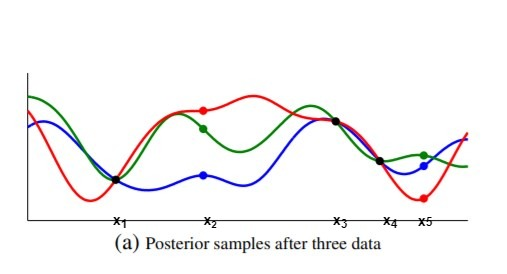
\includegraphics[width=1.\textwidth]{images/parallel/parallel_a.jpg}}
    \only<3-5>{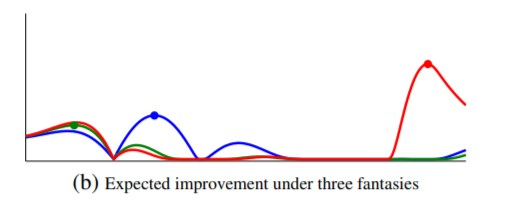
\includegraphics[width=1.\textwidth]{images/parallel/parallel_b.jpg}}
    \only<4-5>{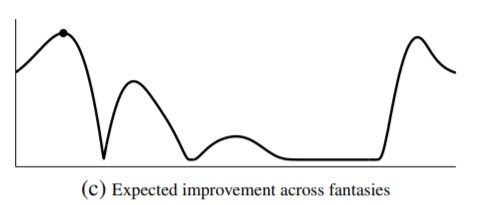
\includegraphics[width=1.\textwidth]{images/parallel/parallel_c.jpg}}
\end{column}%
\end{columns}

\source{Snoek et al. 2012}
\end{frame}
%-----------------------------------------------------------------------
